\newpage
\section{Concluding Remarks}
This work developed a uniquely identifiable parametric hybrid nonlinear model structure for SCR-ASC dynamics based on
first principles. Rather than relying on spatial discretization with multiple CSTR cells, the approach focused on modeling the temporal evolution of key species concentrations using molar conservation principles. The model explicitly accounts for:

\begin{enumerate}
        \item Interplay between residence time and sampling time, ensuring the model captures dynamic effects within observable time scales.
        \item Higher-order polynomial and reciprocal models for physical properties, including residence time and temperature-dependent rate constants, improving model accuracy.
        \item Catalyst saturation and desaturation dynamics, by explicitly modeling $NO_x$ reduction dynamics under each condition, and implementing a switching mechanism between these states.
\end{enumerate}

The parameters of the developed hybrid model are uniquely identifiable from data using convex optimization techniques.
Specifically, the parameters of the saturated model are estimated by solving a linear programming problem that minimizes
the area under the "$NO_x$ reduction per time step under saturation" curve, with a lower bound set by actual $NO_x$
reduction observed in the data. The identified saturated model is then used to detect catalyst desaturation segments,
which inform the parameter estimation of the desaturated model.

Finally, validation against test data demonstrates a significant improvement in capturing system dynamics compared to
traditional linear CSTR models from the literature. The enhanced model accuracy confirms the effectiveness of the
proposed approach in representing SCR-ASC dynamics and provides a strong foundation for improved diagnostics in diesel
after-treatment systems.


\subsection{A review of the problems identified and solved}

During the model development, several issues were identified and addressed. The primary motivation stemmed from the
causality reversal observed when reducing a multi-cell CSTR model to a single cell and linearizing it around operating
conditions. Another significant issue was the strong dependence of the nonlinear model's frequency response on sampling
time, which caused a loss of information when using direct Euler discretization. These issues were resolved by deriving
molar conservation equations from first principles, which revealed the critical relationship between residence time and
sampling time. The final model explicitly incorporates this relationship, ensuring a more accurate and physically
consistent representation of SCR-ASC dynamics.

Another issue involved the parameter estimation. The nonlinear CSTR model not only involved a large number of parameters
but also resulted in a non-convex estimation problem. In contrast, the linearized CSTR model simplified the problem by
producing convex lumped parameters, but it introduced the issues discussed earlier. The discrete model developed in this
work, however, uses polynomial approximations for exponential terms, making the system linear in parameters and ensuring
a more parsimonious and identifiable model.

The initial parametrization approach of the model included states that were not directly measurable, particularly the
surface concentration of adsorbed ammonia. The first approach to address this was through a multi-rate estimation
method. However, it was later discovered that the surface concentration state could be algebraically eliminated by
introducing recursion into the model. This led to the definition of a new state, $\eta(k) = u_1(k-1) - x_1(k)$, which
represents the change in $NO_x$ concentration due to reduction over a given time step. This recursive dynamic model’s
parameters were identifiable using the available measurements.

Finally, catalyst saturation was explicitly introduced, and its model parameters were identified using a linear
programming approach, resulting in a hybrid nonlinear model that switches between saturation and desaturation.

\begin{figure}[H]
        \centering
        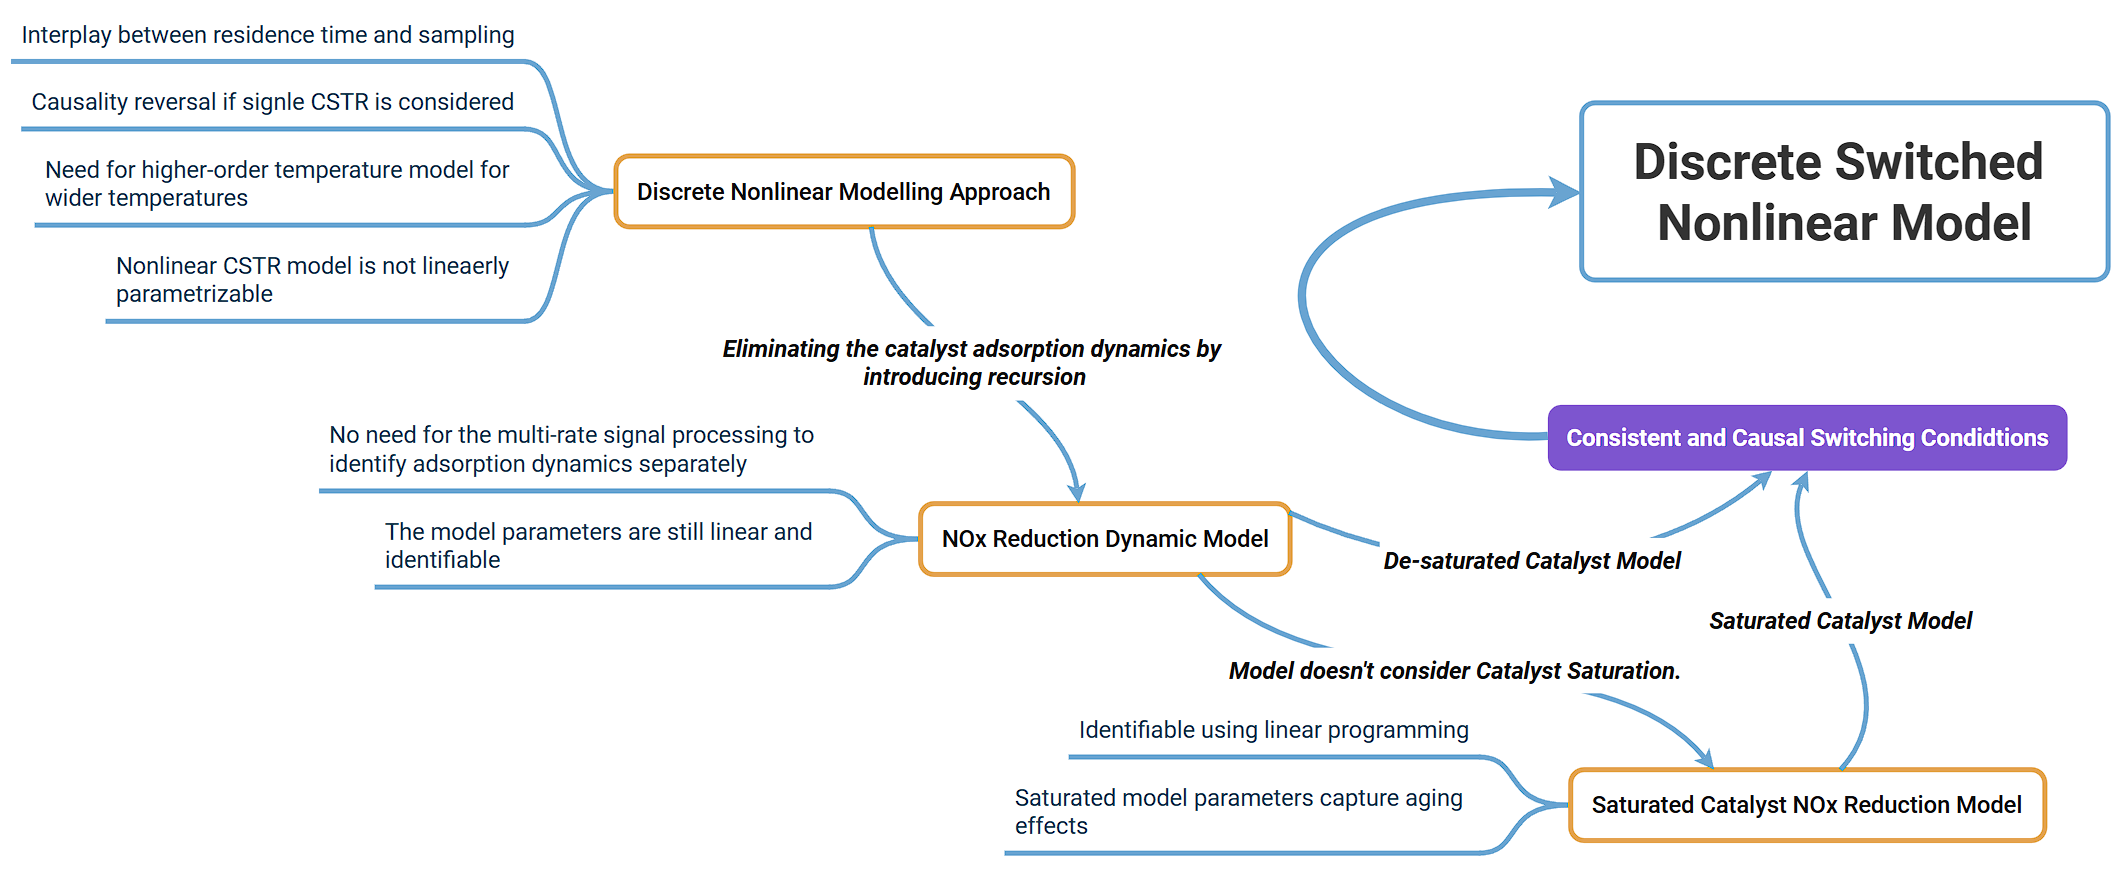
\includegraphics[width = 0.9\textwidth]{\froot/figs/n_figs/problems_soved.png}
        \caption{A map of the developments}
\end{figure}
